\documentclass{article}
% translate with >> pdflatex -shell-escape <file>

% This file is used as unit test for pgfplots, copyright by Christian Feuersaenger.
% 
% See
%   http://pgfplots.sourceforge.net/pgfplots.pdf
% for pgfplots.
%
% Any required input files (for <plot table> or <plot file> or the table package) can be downloaded
% at
% http://www.ctan.org/tex-archive/graphics/pgf/contrib/pgfplots/doc/latex/
% and
% http://www.ctan.org/tex-archive/graphics/pgf/contrib/pgfplots/doc/latex/plotdata/

\usepackage{pgfplots}
\pgfplotsset{compat=1.3}

\pagestyle{empty}

\begin{document}

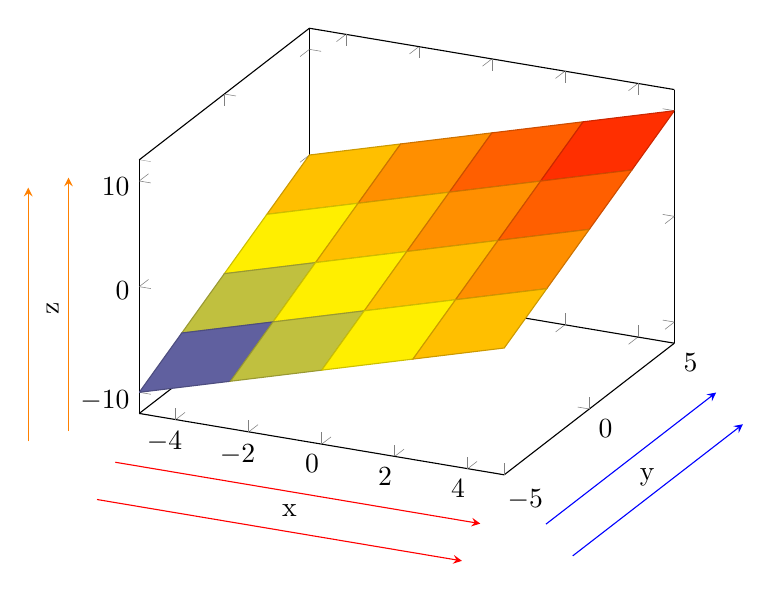
\begin{tikzpicture}
	\begin{axis}[samples=5,xlabel=x,ylabel=y,zlabel=z,
		extra description/.append code={%
			\draw[red,-stealth] (xticklabel cs:0) -- (xticklabel cs:1);
			\draw[red,-stealth] (xticklabel cs:0,15pt) -- (xticklabel cs:1,15pt);
			%
			\draw[blue,-stealth] (yticklabel cs:0) -- (yticklabel cs:1);
			\draw[blue,-stealth] (yticklabel cs:0,15pt) -- (yticklabel cs:1,15pt);
			%
			\draw[orange,-stealth] (zticklabel cs:0) -- (zticklabel cs:1);
			\draw[orange,-stealth] (zticklabel cs:0,15pt) -- (zticklabel cs:1,15pt);
		}]
		\addplot3[surf] {x+y};

	\end{axis}
\end{tikzpicture}
\end{document}
